\documentclass[aspectratio=169]{beamer}
\usepackage[utf8]{inputenc} % codificacao de caracteres
\usepackage[T1]{fontenc}    % codificacao de fontes
\usepackage[english]{babel}  % idioma
\usepackage{graphics,amssymb,amsfonts,amsmath,xfrac}
\usepackage{tikz}
\usepackage{enumerate,hyperref}
\usepackage{palatino}	% Fonte sem serifa
\usepackage{ragged2e}	% Paragrafo justificado
%\usepackage{minted}	% Highlight para codigos de programacao
\usepackage{booktabs} % tabelas
\usepackage{multicol}
\usepackage{multirow}

%\usepackage[table]{xcolor}


% Veja mais temas e cores em http://www.hartwork.org/beamer-theme-matrix/
\usetheme{Montpellier}         % tema
\usecolortheme{orchid}      % cores
\usefonttheme[onlymath]{serif} % fonte modo matematico
% Colocando numero de paginas no slide
\setbeamertemplate{footline}[frame number]



\DeclareGraphicsExtensions{.pdf,.JPG,.png} % compilamos apenas com pdflatex
%\graphicspath{{./figuras/}} % caminho onde as figuras estarao disponiveis


\graphicspath{{figuras/}}

% ---------------------------------------------------------------------------- %
% T�tulo                                                                       %
% ---------------------------------------------------------------------------- %

\title[\sc{Teoria de Circuitos Eletrônicos 1}]{\LARGE Aula 10 - The Complete Response of RL and RC Circuits}
\author[Prof. Marcelino Andrade]{Prof. Marcelino Andrade}
\institute{Faculdade UnB Gama} % opcional
\date{\today}

\begin{document}
\justifying % Paragrafo justificado
\pagebreak

\begin{frame}
  \titlepage
\end{frame}


% ----------------- NOVO SLIDE --------------------------------
\begin{frame}{Contents}

\tableofcontents
%\begin{center}	
     		Introduction to Electric Circuits by James A. Svoboda, Richard C. Dorf, 9th Edition 
  %   		Fundamentals of Electric Circuits by Alexander and Sadiku, 4th Edition	
%\end{center}	
\end{frame}

% ----------------- NOVA SECÇÂO -----------------------------
\section{Introduction (7.1)}
% ----------------- NOVO SLIDE --------------------------------
\begin{frame}[fragile]
	\frametitle{Introduction}
		\begin{tabular}{cc}
			\begin{columns}
				\begin{column}{1\textwidth}  %%<--- here
					In this chapter, we consider the response of RL and RC circuits to abrupt changes. The abrupt change
might be a change to the circuit, as when a switch opens or closes. Consequently, we will do the following:	
		
\small 			\begin{itemize}
						\item[$\clubsuit$]{Develop vocabulary that will help us talk about the response of a first-order circuit.}
						\item[$\clubsuit$]{Analyze first-order circuits with inputs that are constant after some particular time, $t_0$.}
						\item[$\clubsuit$]{Introduce the notion of a stable circuit and use it to identify stable first-order circuits.}	
						\item[$\clubsuit$]{Analyze first-order circuits that experience more than one abrupt change.}	
						\item[$\clubsuit$]{Introduce the step function and use it to determine the step response of a first-order circuit.}	
						\item[$\clubsuit$]{Analyze first-order circuits with inputs that are not constant.}	

					\end{itemize}
					
				\end{column}
			\end{columns}
		
	\end{tabular}
\end{frame}

% ----------------- NOVA SECÇÂO -----------------------------
\section{First-Order Circuits (8.2)}
% ----------------- NOVO SLIDE --------------------------------
\begin{frame}[fragile]
	\frametitle{First-Order Circuits}
		\begin{tabular}{cc}
			\begin{columns}
				\begin{column}{1\textwidth}  %%<--- here
\small					Circuits that contain only one inductor and no capacitors or only one capacitor and no
inductors can be represented by a first-order differential equation. These circuits are called \textbf{first-order circuits}.
%\begin{center}
 \center A plan for analyzing first-order circuits. 
%\end{center}			
				\end{column}
			\end{columns}\\
		
\begin{columns}
	\begin{column}{.5\textwidth}  %%<--- here
	\center			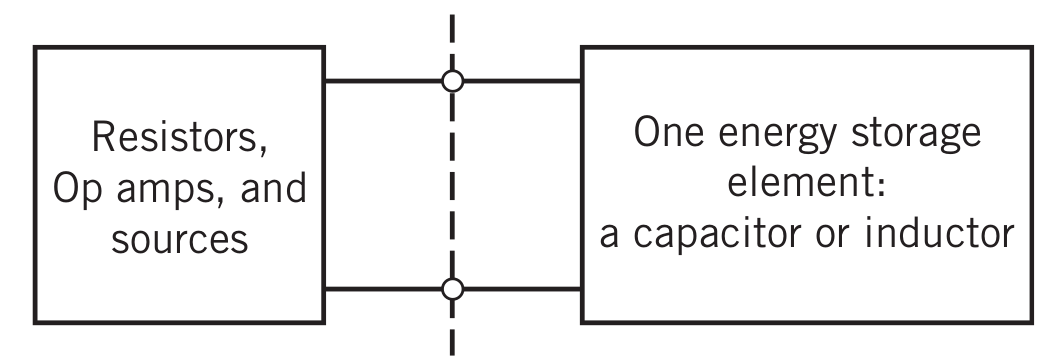
\includegraphics[width=5cm,height=1.5cm]{figure4.png}\\
				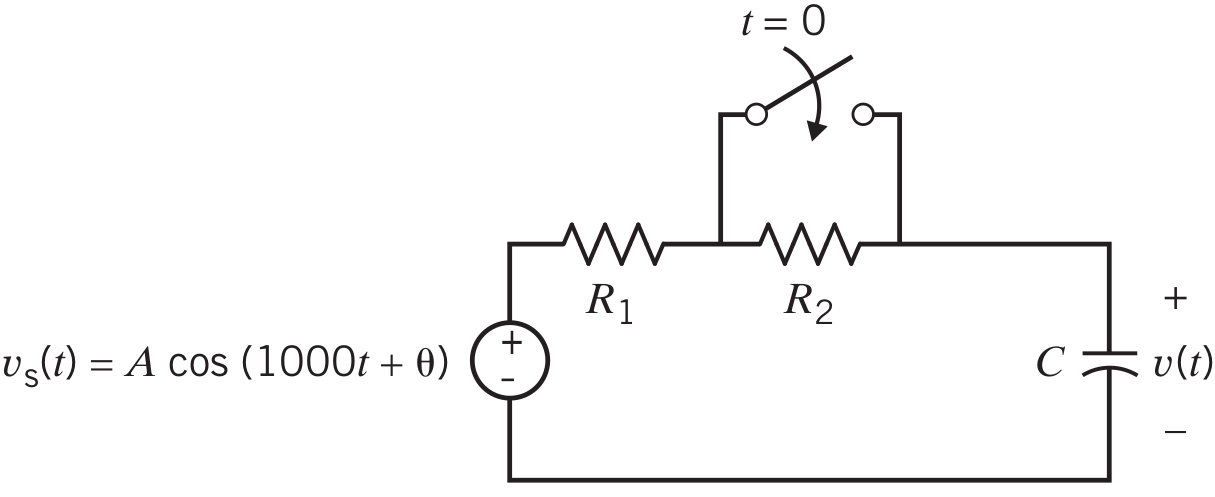
\includegraphics[width=5cm,height=1.5cm]{figure1.png}
				\end{column}
		
	\begin{column}{.5\textwidth}  %%<--- here\
	\center			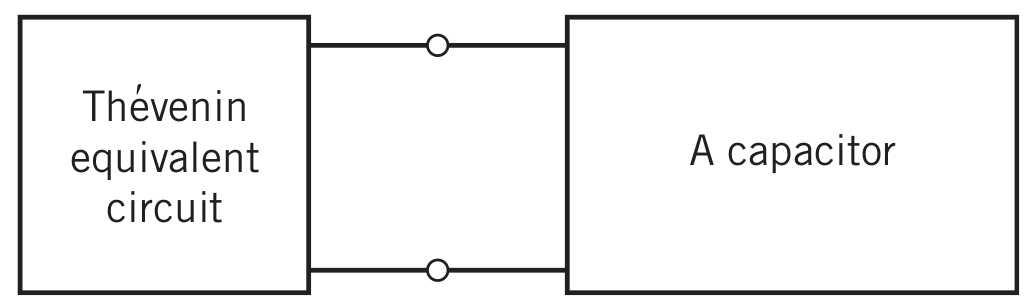
\includegraphics[width=5cm,height=1.5cm]{figure3.png}\\
				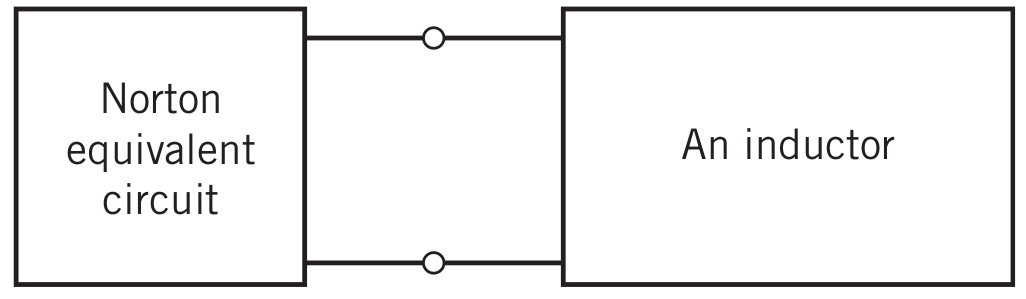
\includegraphics[width=5cm,height=1.5cm]{figure2.png}
		
				\end{column}				
		\end{columns}\\
		
\begin{columns}
	\begin{column}{.5\textwidth}  %%<--- here
\tiny					First, separate the energy storage element from the
rest of the circuit.
		
				\end{column}
		
	\begin{column}{.5\textwidth}  %%<--- here
\tiny					Next, replace the circuit connected
to a capacitor by its Thevenin equivalent circuit or
replace the circuit connected to an inductor by its Norton
equivalent circuit.
		
				\end{column}		
		
		
		
		\end{columns}\\		
		
		
		
		
	\end{tabular}	
	
	
	
	
	
	
\end{frame}
% ----------------- NOVO SLIDE --------------------------------
\begin{frame}[fragile]
	\frametitle{First-Order Circuits}
		\begin{tabular}{cc}
			\begin{columns}
				\begin{column}{1\textwidth}  %%<--- here
\small					After the switch closes, the response will consist of two parts: a transient part that eventually dies out
and a steady-state part. 
%\end{center}			
				\end{column}
			\end{columns}\\
		
\begin{columns}
	\begin{column}{.5\textwidth}  %%<--- here
	\center			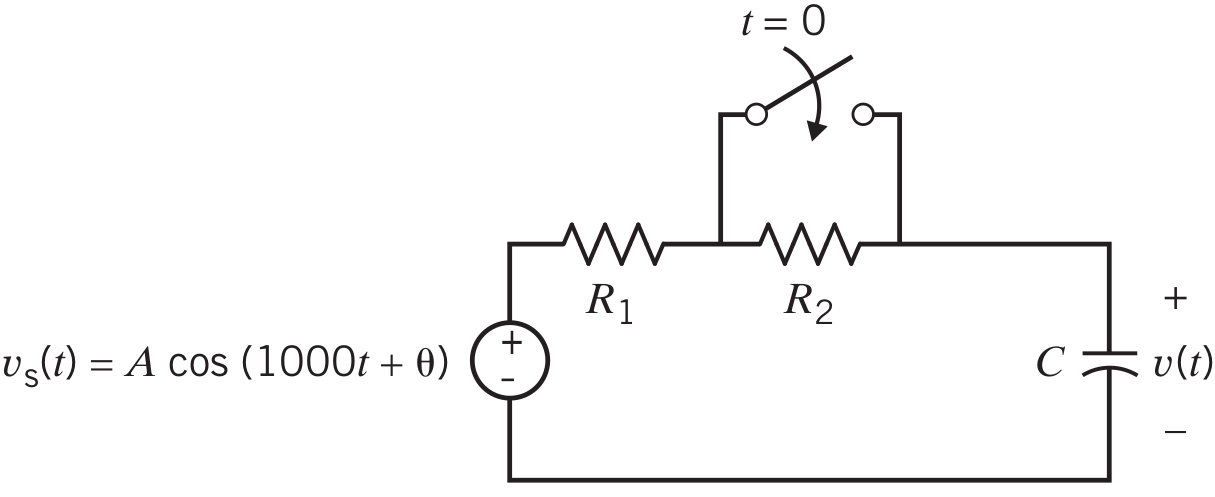
\includegraphics[width=6cm,height=3.0cm]{figure1.png}
				
				\end{column}
		
	\begin{column}{.5\textwidth}  %%<--- here\
	\center			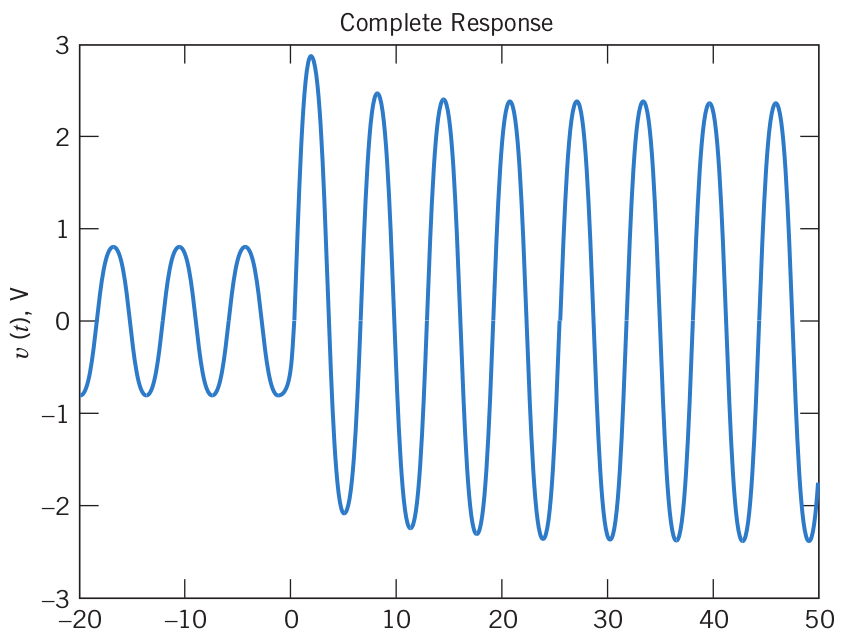
\includegraphics[width=5cm,height=3cm]{figure5.png}
		
				\end{column}				
		\end{columns}\\
		
\begin{columns}
	\begin{column}{.5\textwidth}  %%<--- here
\center \small					Complete  Response $=$ Transient Response $+$ Steady-State  Response
		
				\end{column}
		
	\begin{column}{.5\textwidth}  %%<--- here
\center \small					$v(t)=Ke^{\frac{-t}{\tau}}+M \cos(1000t+\delta)$
		
				\end{column}		
		
		
		
		\end{columns}\\		
		
		
		
		
	\end{tabular}	
	
	
	
	
	
	
\end{frame}
% ----------------- NOVA SECÇÂO -----------------------------


\begin{frame}[fragile]
	\frametitle{First-Order Circuits}
		\begin{tabular}{cc}
			\begin{columns}
				\begin{column}{1\textwidth}  %%<--- here
In general, the \textbf{complete response} of a first-order circuit can be represented as the sum of two
parts, the natural response and the forced response:

%\end{center}			
				\end{column}
			\end{columns}\\
		
\begin{columns}
	\begin{column}{1\textwidth}  %%<--- here
\center \textbf{Complete Response} $=$ \textbf{Natural Response} $+$ \textbf{Forced Response} \newline
\small		\begin{itemize}
\item The \textbf{natural response} is the source free solution and the initial condition is not neglected. 
\item The \textbf{forced response} is not the source free solution and the initial condition is neglected.			 
		\end{itemize}		
				\end{column}
		\end{columns}\\

		\begin{columns}
	\begin{column}{1\textwidth}  %%<--- here
\newline \newline  \small The complete response of a first-order circuit will depend on an initial condition, usually a
capacitor voltage or an inductor current at a particular time.
				\end{column}
		\end{columns}

		
	\end{tabular}	
	
\end{frame}

% ----------------- NOVO SLIDE --------------------------------


\begin{frame}[fragile]
	\frametitle{First-Order Circuits}
		\begin{tabular}{cc}
			\begin{columns}
				\begin{column}{1\textwidth}  %%<--- here
In general, the \textbf{complete response} of a first-order circuit can be represented as the sum of two
parts, the natural response and the forced response:

%\end{center}			
				\end{column}
			\end{columns}\\
		
\begin{columns}
	\begin{column}{1\textwidth}  %%<--- here
\center \textbf{Plan for finding the complete response of first-order circuits} 
\small		\begin{enumerate}
					\item {\small Obtain the initial condition of the energy storage element.}
					\item { \small  Find the natural response after the disturbance.}
					\item { \small  Find the forced response after the disturbance.}
					\item { \small  Add the natural response to the forced response to get the complete response.}	

					\end{enumerate}
			
				\end{column}
		\end{columns}\\

	
	
	\begin{columns}
	\begin{column}{1\textwidth}  %%<--- here
\newline \newline  \small Use the initial condition to obtain natural response.
	
			
				\end{column}
		\end{columns}\\
	
		
	\end{tabular}	
	
\end{frame}

% ----------------- NOVA SECÇÂO -----------------------------

\section{The Response of a First-Order Circuit to a Constant Input (8.3)}
% ----------------- NOVO SLIDE --------------------------------
\begin{frame}[fragile]
	\frametitle{The Response of a First-Order Circuit to a Constant Input}

		\begin{tabular}{cc}
			\begin{columns}
				\begin{column}{1\textwidth}  %%<--- here
\small					In this section, we find the complete response of a first-order circuit when the input to the circuit is
constant after time $t_0$ . 
%\end{center}			
				\end{column}
			\end{columns}\\
		
\begin{columns}
	\begin{column}{.5\textwidth}  %%<--- here
	\center			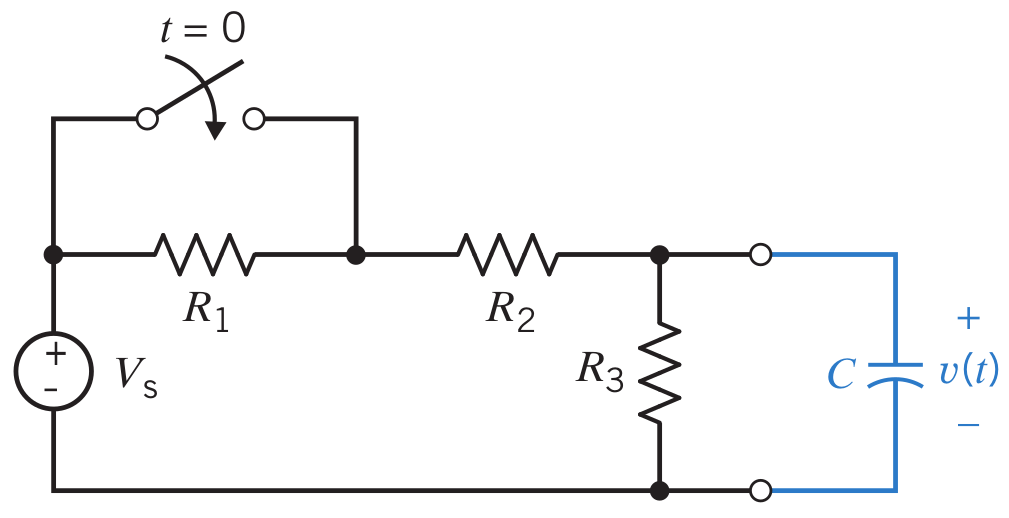
\includegraphics[width=5cm,height=2.0cm]{figure6.png} \\
\tiny	A first-order circuit containing a capacitor.
				
				\end{column}
		
	\begin{column}{.5\textwidth}  %%<--- here\
	\center			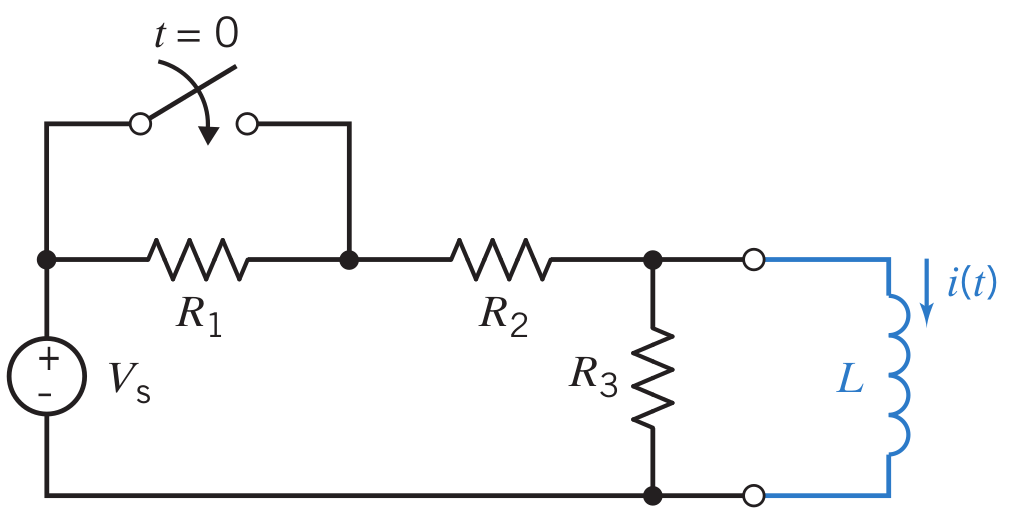
\includegraphics[width=5cm,height=2cm]{figure8.png} \\
\tiny	A first-order circuit containing an inductor.	
				\end{column}				
		\end{columns}\\
		
\begin{columns}
	\begin{column}{.5\textwidth}  %%<--- here

	
\begin{columns}	
	\begin{column}{.4\textwidth}
	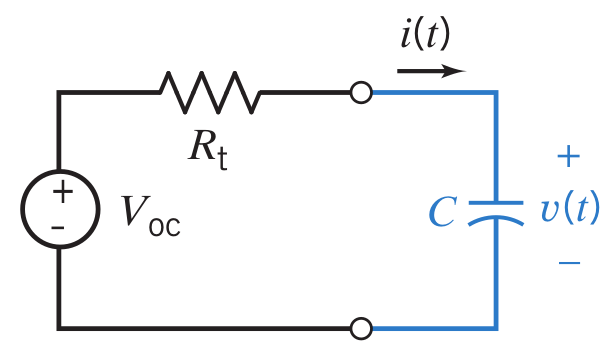
\includegraphics[width=3cm,height=1.5cm]{figure7.png}
	\end{column}
	\begin{column}{.4\textwidth}
\tiny $V_{oc}=\frac{R_3}{R_3+R_2}V_s $ 
\newline \newline
\tiny $R_{t}=\frac{R_2R_3}{R_2+R_3}$
	\end{column}
\end{columns}


\center \tiny After the switch closes, the circuit connected to the capacitor is replaced by its Thevenin equivalent circuit.
				
				\end{column}
		
	\begin{column}{.5\textwidth}  %%<--- here

	\begin{columns}	
	\begin{column}{.4\textwidth}
	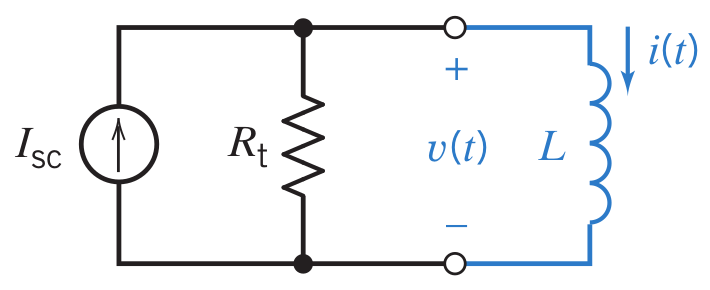
\includegraphics[width=3cm,height=1.5cm]{figure9.png}
	\end{column}
	\begin{column}{.4\textwidth}
\tiny $I_{sc}=\frac{V_s}{R_2}$ 
\newline \newline
\tiny $R_{t}=\frac{R_2R_3}{R_2+R_3}$
	\end{column}
\end{columns}
	\center	\tiny After the switch closes, the circuit connected to the inductor is replaced by its Norton equivalent circuit.				
				\end{column}		
		\end{columns}\\		
	\end{tabular}	
	
\end{frame}
% ----------------- NOVO SLIDE --------------------------------
\begin{frame}[fragile]
	\frametitle{The Response of a First-Order Circuit to a Constant Input}

		\begin{tabular}{cc}
			\begin{columns}
				\begin{column}{.5\textwidth}  %%<--- here
	\center			  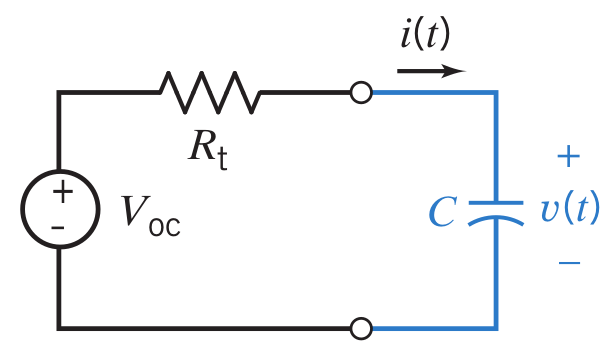
\includegraphics[width=3cm,height=1.5cm]{figure7.png}
				\end{column}
				\begin{column}{.5\textwidth}  %%<--- here
	\center			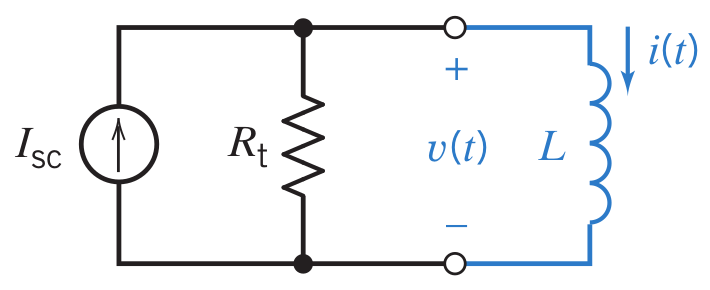
\includegraphics[width=3cm,height=1.2cm]{figure9.png}
				\end{column}
			\end{columns}\\	
				\begin{columns}
				\begin{column}{.5\textwidth}  %%<--- here
\footnotesize	\begin{eqnarray}	 \nonumber	-V_{oc}+R_ti(t)+v(t)&=&0 \\ \nonumber 
				-V_{oc}+R_tC\frac{d}{dt}v(t)+v(t)&=&0 \\  
				\frac{d}{dt}v(t)+\frac{v(t)}{R_tC}&=&\frac{V_{oc}}{R_tC}
	\end{eqnarray}
				\end{column}
				\begin{column}{.5\textwidth}  %%<--- here
\footnotesize	\begin{eqnarray}  \nonumber	-I_{sc}+\frac{v(t)}{R_t}+i(t)&=&0 \\  \nonumber
				-I_{sc}+\frac{L}{R_t}\frac{d}{dt}i(t)+i(t)&=&0 \\   
				\frac{d}{dt}i(t)+\frac{i(t)}{\sfrac{L}{R_t}}&=&\frac{I_{sc}}{\sfrac{L}{R_t}}
	\end{eqnarray}
				\end{column}
			\end{columns}\\	
			\begin{columns}
				\begin{column}{1\textwidth}  %%<--- here
\footnotesize		\center	 The parameter $\tau$ is called time constant and both equations have the same form. That is \newline \newline
\normalsize	$\frac{d}{dt}x(t)+\frac{x(t)}{\tau}=K$\\

				\end{column}
	
			\end{columns}\\	
					
\end{tabular}	
	
\end{frame}

% ----------------- NOVO SLIDE --------------------------------
\begin{frame}[fragile]
	\frametitle{The Response of a First-Order Circuit to a Constant Input}

		\begin{tabular}{cc}
				\begin{columns}
				\begin{column}{1\textwidth}  %%<--- here
\small	We will solve the differential equation below by separating the
variables and integrating. Then we will use the solution of Eqs. 3 to obtain solutions of Eqs. 1
and 2. \newline
				\end{column}
			\end{columns}\\	

				\begin{columns}
				\begin{column}{.2\textwidth}  %%<--- here
\footnotesize	\begin{eqnarray}	 	
			  \frac{d}{dt}x(t)+\frac{x(t)}{\tau}&=&K \\ \nonumber
			  \frac{dx}{dt}&=& \frac{K \tau-x}{\tau} \\ \nonumber
			  \frac{dx}{x-K \tau}&=& -\frac{dt}{\tau} \\ \nonumber
			 \int \frac{dx}{x-K \tau}&=& -\int \frac{dt}{\tau} + D\\ \nonumber
			 \int \frac{dx}{x-K \tau}&=& -\frac{1}{\tau} \int dt + D\\ \nonumber
	\end{eqnarray}
				\end{column}
				\begin{column}{.8\textwidth}  %%<--- here
\footnotesize	\begin{eqnarray}	 	
	\nonumber		 \ln(x-K \tau)&=& -\frac{t}{\tau} + D\\ \nonumber
			  x(t)&=&K\tau+A e^{-\frac{t}{\tau}} \ and \ A=e^D \\ \nonumber
			  To \ find \ A, let \ t=0. \ Then \\ \nonumber
			  x(0)&=&K\tau+A e^{-\frac{0}{\tau}} \\ \nonumber
			 A&=& x(0)-K\tau \\ \nonumber
			 Because, \ x(\infty)=K\tau\\ 
			 x(t)&=&x(\infty)+(x(0)-x(\infty)) e^{-\frac{t}{\tau}} \\ \nonumber
	\end{eqnarray}
				\end{column}
			\end{columns}\\	

					
\end{tabular}	
	
\end{frame}
% ----------------- NOVO SLIDE --------------------------------
\begin{frame}[fragile]
	\frametitle{The Response of a First-Order Circuit to a Constant Input}

		\begin{tabular}{cc}
				\begin{columns}
				\begin{column}{1\textwidth}  %%<--- here
\scriptsize Then we will use the Eqs. 4 to obtain solutions of Eqs. 1 and 2.
				\end{column}
			\end{columns}\\	
				\begin{columns}
				\begin{column}{.5\textwidth}  %%<--- here
			\center			  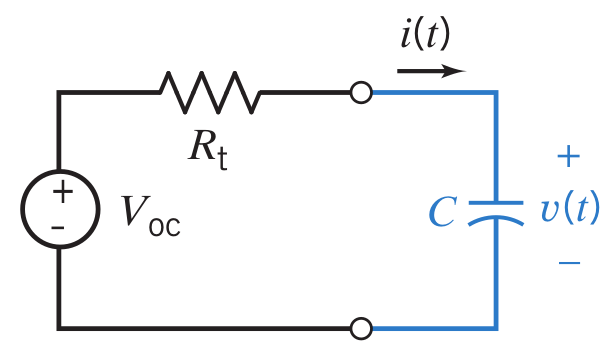
\includegraphics[width=3cm,height=1.5cm]{figure7.png}
		\scriptsize	 $\frac{d}{dt}v(t)+\frac{v(t)}{R_tC}=\frac{V_{oc}}{R_tC}$ 
\scriptsize	\begin{eqnarray}
	\nonumber	  \frac{d}{dt}x(t)+\frac{x(t)}{\tau}&=&K \\ \nonumber
			 x(t)&=&x(\infty)+(x(0)-x(\infty)) e^{-\frac{t}{\tau}} \\ \nonumber
			  v(t)&=&V_{oc}+(v(0)-v_{oc}) e^{-\frac{t}{R_tC}}  \nonumber
	\end{eqnarray}
\scriptsize	Complete response $v(t)$, Steady-State  Response $V_{oc}$ and 
Transient Response $(v(0)-v_{oc}) e^{-\frac{t}{R_tC}}$
	
	
				\end{column}
				\begin{column}{.5\textwidth}  %%<--- here
					\center			  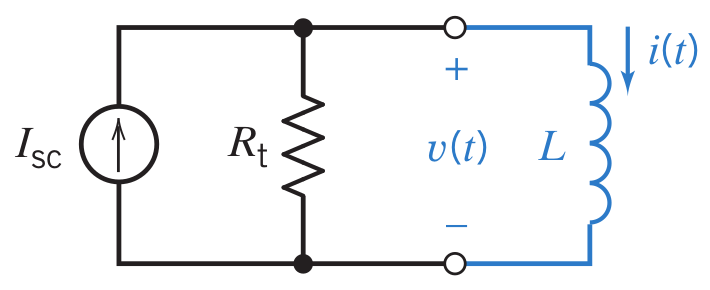
\includegraphics[width=3cm,height=1.5cm]{figure9.png}
			\scriptsize		$\frac{d}{dt}i(t)+\frac{i(t)}{\sfrac{L}{R_t}}=\frac{I_{sc}}{\sfrac{L}{R_t}}$
\scriptsize	\begin{eqnarray}
	\nonumber	  \frac{d}{dt}x(t)+\frac{x(t)}{\tau}&=&K \\ \nonumber
			 x(t)&=&x(\infty)+(x(0)-x(\infty)) e^{-\frac{t}{\tau}} \\ \nonumber
			  i(t)&=&I_{sc}+(i(0)-I_{sc}) e^{-\frac{t}{\sfrac{L}{R_t}}}
	\end{eqnarray}
	\scriptsize	Complete response $i(t)$, Steady-State  Response $I_{sc}$ and 
Transient Response $(i(0)-I_{sc}) e^{-\frac{t}{\sfrac{L}{R_t}}}$
				\end{column}
			\end{columns}\\	

					
\end{tabular}	
	
\end{frame}
% ----------------- NOVO SLIDE --------------------------------
\begin{frame}[fragile]
	\frametitle{The Response of a First-Order Circuit to a Constant Input}

		\begin{tabular}{cc}
				\begin{columns}
				\begin{column}{1\textwidth}  %%<--- here
\scriptsize Then we will use the Eqs. 4 to obtain solutions of Eqs. 1 and 2.
				\end{column}
			\end{columns}\\	
				\begin{columns}
				\begin{column}{.5\textwidth}  %%<--- here
			\center			  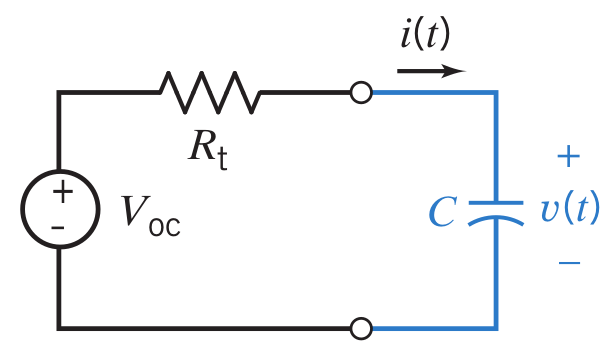
\includegraphics[width=3cm,height=1.5cm]{figure7.png}
		\scriptsize	 $\frac{d}{dt}v(t)+\frac{v(t)}{R_tC}=\frac{V_{oc}}{R_tC}$ 
$v(t)=V_{oc}+(v(0)-V_{oc}) e^{-\frac{t}{R_tC}}$
\begin{center} \scriptsize	Complete response $v(t)$, Steady-State  Response $V_{oc}$ and 
Transient Response $(v(0)-V_{oc}) e^{-\frac{t}{R_tC}}$ \end{center} 
$v(t)=V_{oc}(1- e^{-\frac{t}{R_tC}})+v(0) e^{-\frac{t}{R_tC}}$ \\
\begin{center} \scriptsize	Complete response $v(t)$, forced response $V_{oc}(1- e^{-\frac{t}{R_tC}})$ and 
natural response $v(0) e^{-\frac{t}{R_tC}}$ \end{center}
	
	
				\end{column}
				\begin{column}{.5\textwidth}  %%<--- here
					\center			  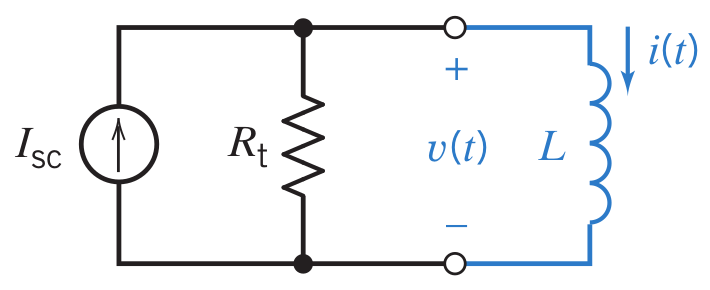
\includegraphics[width=3cm,height=1.5cm]{figure9.png}
			\scriptsize		$\frac{d}{dt}i(t)+\frac{i(t)}{\sfrac{L}{R_t}}=\frac{I_{sc}}{\sfrac{L}{R_t}}$
 $i(t)=I_{sc}+(i(0)-I_{sc}) e^{-\frac{t}{\sfrac{L}{R_t}}}$
\begin{center}	\scriptsize	Complete response $i(t)$, Steady-State  Response $I_{sc}$ \\ and 
Transient Response $(i(0)-I_{sc}) e^{-\frac{t}{\sfrac{L}{R_t}}}$ \end{center} 
$i(t)=I_{sc}(1-e^{-\frac{t}{\sfrac{L}{R_t}}})+i(0)e^{-\frac{t}{\sfrac{L}{R_t}}}$
\begin{center} \scriptsize	Complete response $i(t)$, forced response \\ $I_{sc}(1-e^{-\frac{t}{\sfrac{L}{R_t}}})$ and 
natural response $i(0)e^{-\frac{t}{\sfrac{L}{R_t}}}$ \end{center}
				\end{column}
			\end{columns}\\	

					
\end{tabular}	
	
\end{frame}
% ----------------- NOVO SLIDE --------------------------------
\begin{frame}[fragile]
	\frametitle{First-Order Circuit to a Constant Input}
\begin{tabular}{ll}
	\begin{columns}
		\begin{column}{1\textwidth}  %%<--- here
		\textbf{EXAMPLE 8.3-1} - Find the capacitor voltage after the switch opens in the circuit shown in Figure below. What is the value of the
capacitor voltage $50ms$ after the switch opens?\\
		\begin{center}
    			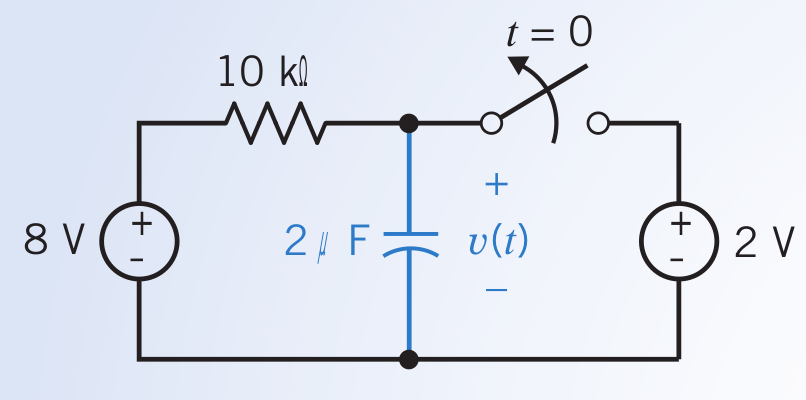
\includegraphics[height=3cm]{figure10.png}	
		\end{center}	
		\scalebox{0.8}{Answer: $v(50)=8-6e^{-\frac{50}{20}}=7.51V \ and \  t[ms].$}
		\end{column}
	\end{columns}
\end{tabular}
\end{frame}

% ----------------- NOVO SLIDE --------------------------------
\begin{frame}[fragile]
	\frametitle{First-Order Circuit to a Constant Input}
\begin{tabular}{ll}
	\begin{columns}
		\begin{column}{1\textwidth}  %%<--- here
		\textbf{EXAMPLE 8.3-4} - The switch in Figure below has been open for a long time, and the circuit has reached steady state before the switch
closes at time $t=0$. Find the inductor current for $t \geq 0$.\\
		\begin{center}
    			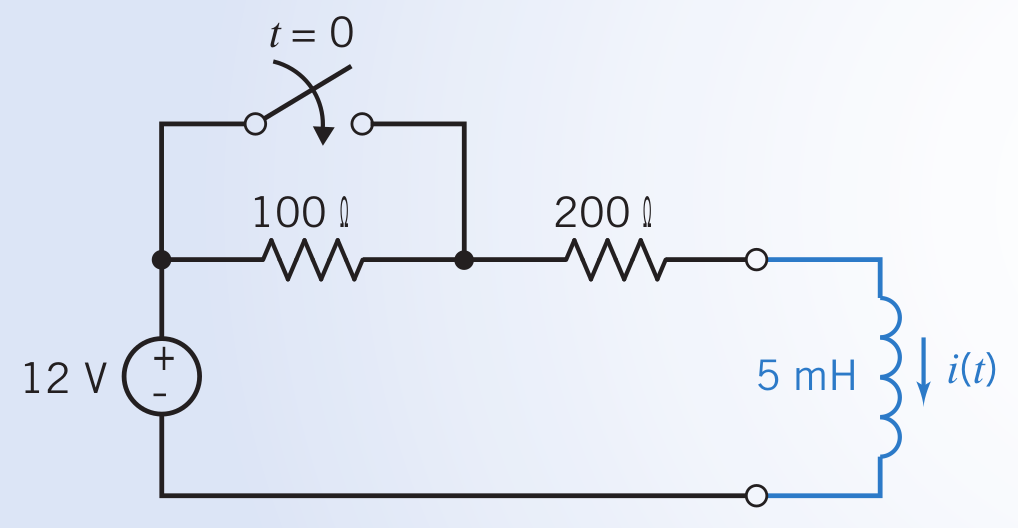
\includegraphics[height=3cm]{figure11.png}	
		\end{center}	
		\scalebox{0.8}{Answer: $i(t)=60-20e^{-\sfrac{t}{25}} mA\ and \  t[\mu s].$}
		\end{column}
	\end{columns}
\end{tabular}
\end{frame}
% ----------------- NOVO SLIDE --------------------------------
\begin{frame}[fragile]
	\frametitle{First-Order Circuit to a Constant Input}
\begin{tabular}{ll}
	\begin{columns}
		\begin{column}{1\textwidth}  %%<--- here
		\textbf{EXAMPLE 8.3-5}- The circuit in Figure below is at steady state before the switch opens. Find the current $i(t)$ for $t > 0$.\\
		\begin{center}
    			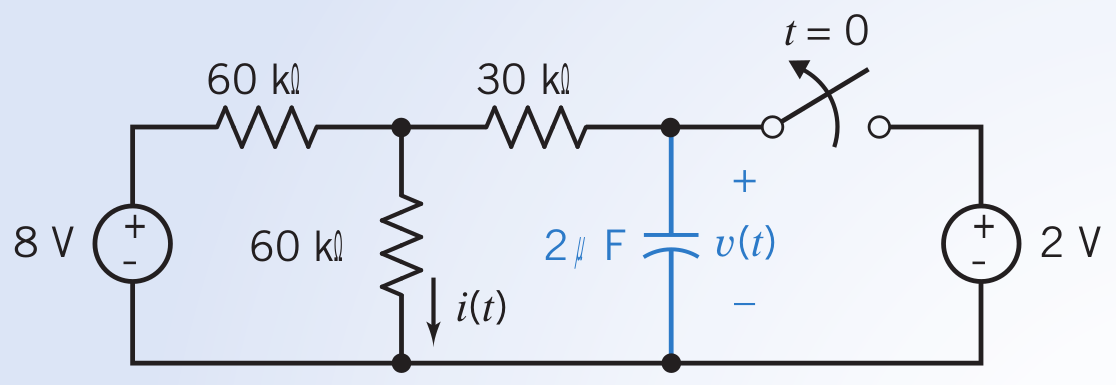
\includegraphics[height=3cm]{figure12.png}	
		\end{center}	
		\scalebox{0.8}{Answer: $i(t)=66.7-16.7e^{-\frac{t}{120}} \mu A\ and \  t[ms].$}
		\end{column}
	\end{columns}
\end{tabular}
\end{frame}
% ----------------- NOVO SLIDE --------------------------------
\begin{frame}[fragile]
	\frametitle{First-Order Circuit to a Constant Input}
\begin{tabular}{ll}
	\begin{columns}
		\begin{column}{1\textwidth}  %%<--- here
		\textbf{EXAMPLE 8.3-7}- Find the inductor current after the switch closes in the circuit shown in Figure below. 
		How long will it take for the inductor current to reach $2 \ mA$?\\
		\begin{center}
    			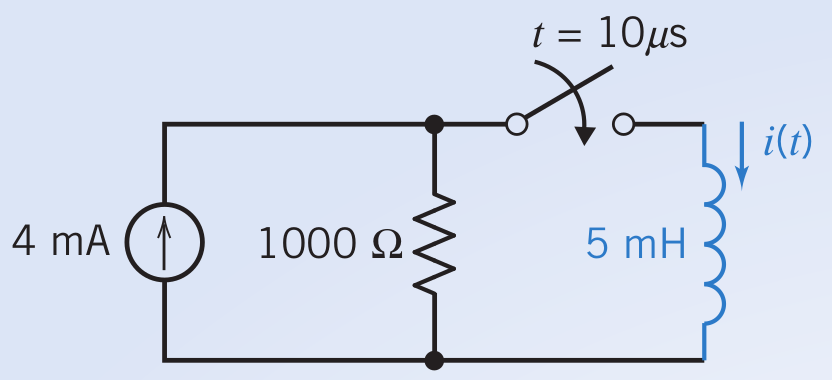
\includegraphics[height=3cm]{figure13.png}	
		\end{center}
		\scalebox{0.8}{Answer: $t=13.47 \mu s $}

		\end{column}
	\end{columns}
\end{tabular}
\end{frame}
% ----------------- NOVO SLIDE --------------------------------
\begin{frame}[fragile]
	\frametitle{First-Order Circuit to a Constant Input}
\begin{tabular}{ll}
	\begin{columns}
		\begin{column}{1\textwidth}  %%<--- here
		\textbf{EXERCISE 8.3-1}- The circuit shown in Figure below is at steady state before the switch closes at time $t=0$.
Determine the capacitor voltage $v(t)$ for $t \geq 0$.\\
		\begin{center}
    			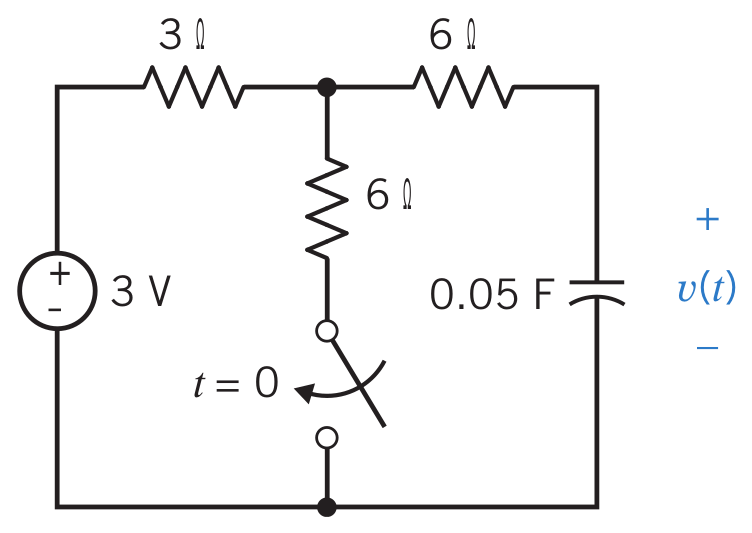
\includegraphics[height=3cm]{figure14.png}	
		\end{center}	
		\scalebox{0.8}{Answer: $v(t)=2-e^{-\frac{t}{0.4}} \ V \ for \ t>0 $}
		\end{column}
	\end{columns}
\end{tabular}
\end{frame}
% ----------------- NOVO SLIDE --------------------------------
\begin{frame}[fragile]
	\frametitle{Calculating the time constant}

		\begin{tabular}{cc}
		\begin{columns}
				\begin{column}{1\textwidth}  %%<--- here
				 	A graphical technique for
measuring the time constant of a first-order circuit.
				\end{column}
						\end{columns}\\		

				\begin{columns}
				\begin{column}{.5\textwidth}  %%<--- here
\small	\begin{eqnarray}
	\nonumber Equation \ (4),\\
	\nonumber	 x(t)&=&x(\infty)+(x(0)-x(\infty)) e^{-\frac{t}{\tau}}\\ 
	\nonumber Derivative \ of\ x(t) \\
	\nonumber	\frac{d}{dx}x(t) \Big|_{t=0}&=& -\frac{1}{\tau}(x(0)-x(\infty)) e^{-\frac{t}{\tau}} \Big|_{t=0} \\ 	\nonumber
	\end{eqnarray} 
\begin{center}
 \LARGE $\tau = \frac{x(\infty)-x(0)}{\frac{d}{dx}x(t)  \Big|_{t=0}}$
\end{center}				\end{column}
				\begin{column}{.4\textwidth}  %%<--- here
					\center			  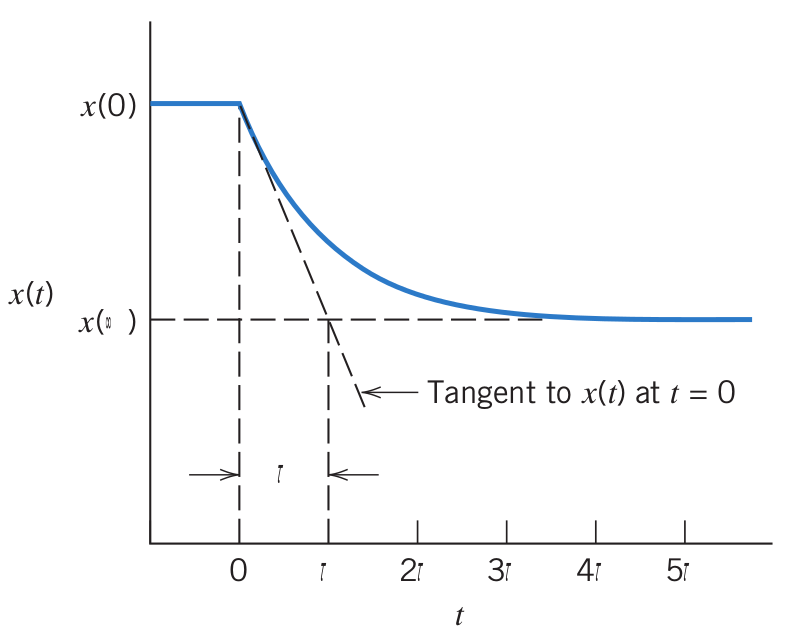
\includegraphics[width=6cm,height=4.5cm]{figure15.png}

				\end{column}
			\end{columns}\\	

					
\end{tabular}	
\end{frame}
% ----------------- NOVA SECÇÂO -----------------------------
\section{Sequential Switching (8.4)}
% ----------------- NOVO SLIDE --------------------------------
\begin{frame}[fragile]
	\frametitle{Sequential Switching}
\begin{tabular}{ll}
	\begin{columns}
		\begin{column}{1\textwidth}  %%<--- here
		\textbf{Sequential switching} occurs when a circuit contains two or more switches that change state at
different instants. As an example of sequential switching, consider the circuit shown in Figure below:\\
		\begin{center}
    			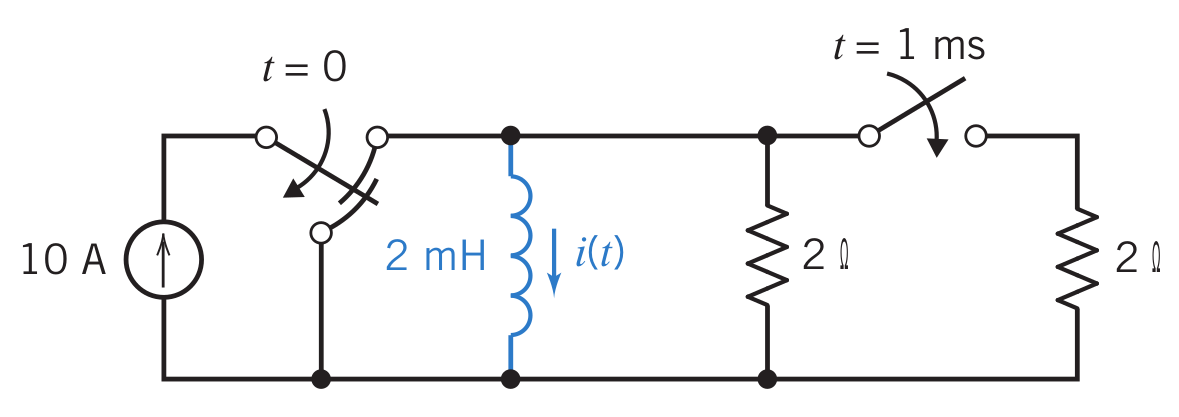
\includegraphics[height=3cm]{figure16.png}	
		\end{center}	
		\scalebox{0.8}{Answer: $i(t)=10e^{-1}e^{-\frac{t-1}{2}} \ A, \ t>1ms\  and \  t[ms].$}
		\end{column}
	\end{columns}
\end{tabular}	
\end{frame}
% ----------------- NOVA SECÇÂO -----------------------------
\section{Stability of First-Order Circuits (8.5)}
% ----------------- NOVO SLIDE --------------------------------
\begin{frame}[fragile]
	\frametitle{Stability of First-Order Circuits}
\begin{tabular}{ll}
	\begin{columns}
		\begin{column}{1\textwidth}  %%<--- here
How can we design first-order circuits to be stable?
		\end{column}
	\end{columns}\\



	\begin{columns}
		\begin{column}{.5\textwidth}  %%<--- here
		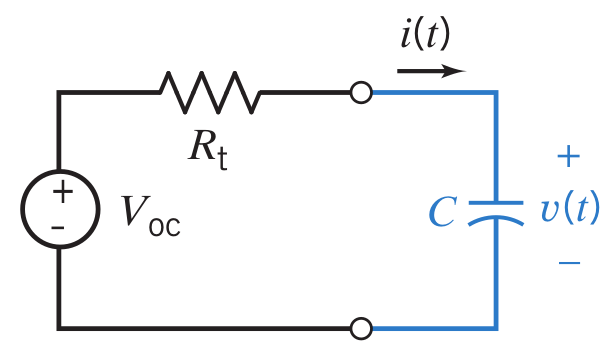
\includegraphics[width=3cm,height=1.5cm]{figure7.png} \scriptsize $v(t)=V_{oc}+(v(0)-V_{oc}) e^{-\frac{t}{R_tC}}$
\begin{center} \scriptsize	Complete response $v(t)$, Steady-State  Response $V_{oc}$ and 
Transient Response $(v(0)-V_{oc}) e^{-\frac{t}{R_tC}}$ \end{center} 
		  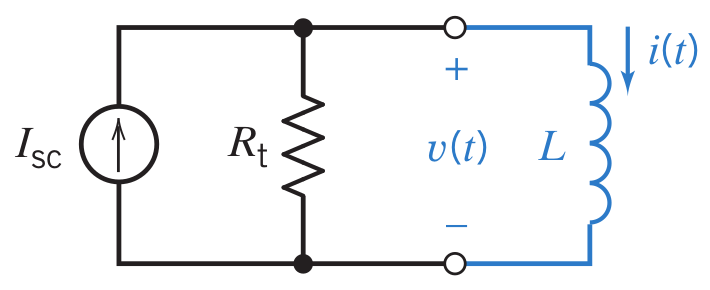
\includegraphics[width=3cm,height=1.5cm]{figure9.png} \scriptsize  $i(t)=I_{sc}+(i(0)-I_{sc}) e^{-\frac{t}{\sfrac{L}{R_t}}}$
\begin{center}	\scriptsize	Complete response $i(t)$, Steady-State  Response $I_{sc}$ \\ and 
Transient Response $(i(0)-I_{sc}) e^{-\frac{t}{\sfrac{L}{R_t}}}$ \end{center} 
		
		\end{column}

		\begin{column}{.5\textwidth}  %%<--- here
\scriptsize		\textbf{\textit{Response}}: Recalling that $\tau=R_tC$ or $\tau=\frac{L}{R_t}$, we see that $R_t > 0$ is required to make a first-order circuit stable.
\newline \newline
\scriptsize		\textbf{EXAMPLE 8.5-1} - The first-order circuit shown in Figure below is at steady state before the switch closes at $t < 0$. 
Find the capacitor voltage $v(t)$ for $t > 0$.\\
		\begin{center}
    			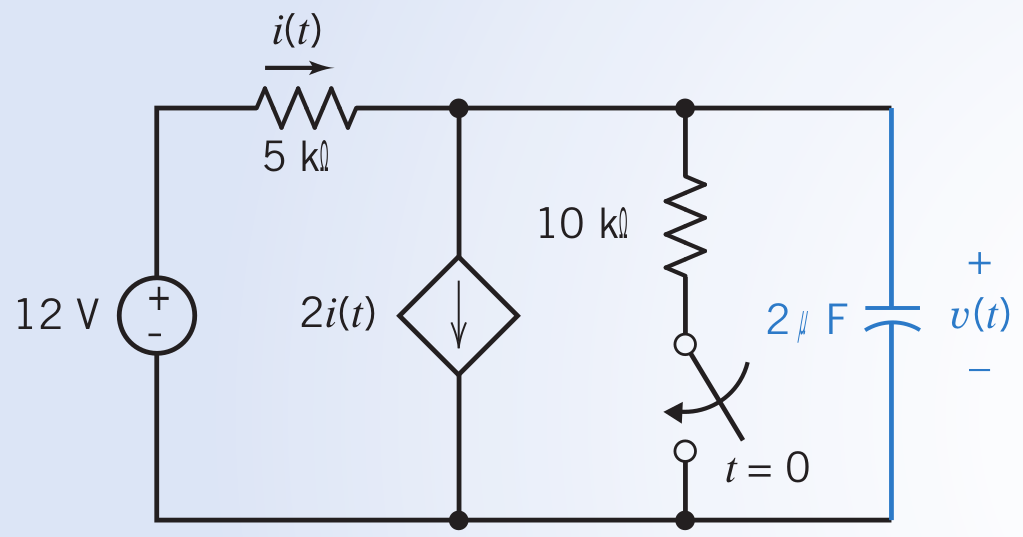
\includegraphics[height=2cm]{figure17.png}	
		\end{center}	
		\scalebox{0.8}{Answer: $v(t)=24-12e^{\sfrac{t}{20}} mA,  \ where \ t \ has\ units\ of\  ms.$}	
		
		\end{column}
	\end{columns}
	
\end{tabular}	
\end{frame}
% ----------------- NOVO SLIDE --------------------------------
\begin{frame}[fragile]
	\frametitle{Stability of First-Order Circuits}
\begin{tabular}{ll}
	\begin{columns}
		\begin{column}{1\textwidth}  %%<--- here
\small		\textbf{EXERCISE 8.5-2}- The circuit considered before has been redrawn in Figure below, with the gain of the dependent
source represented by the variable B. What restrictions must be placed on the gain of the dependent source to
ensure that it is stable? Design this circuit to have a time constant of +20 ms.\\
		\begin{center}
    			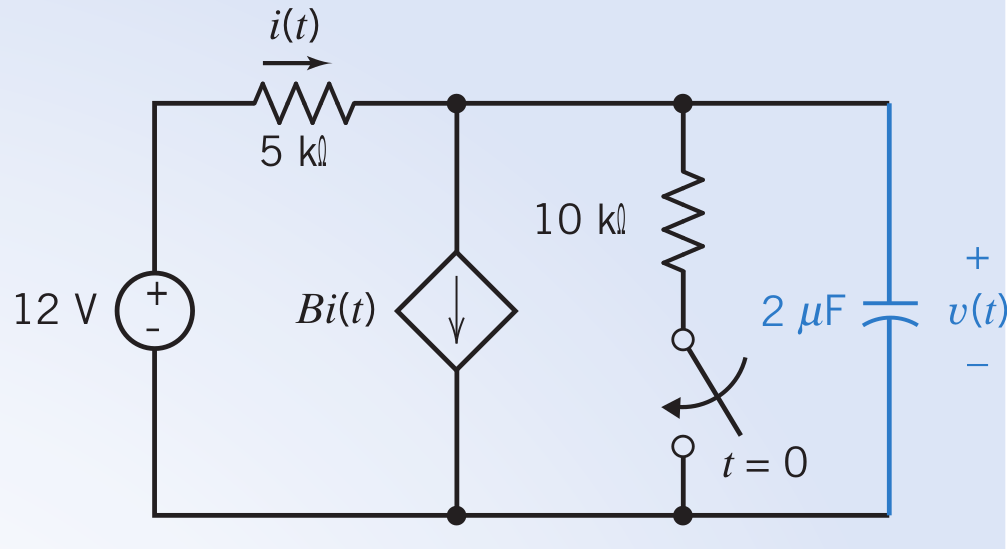
\includegraphics[height=3cm]{figure18.png}	
		\end{center}	
		\scalebox{0.8}{Answer: $B<\frac{3}{2} \ and \ R_t=10K\Omega.$}
		\end{column}
	\end{columns}
\end{tabular}
\end{frame}



% ----------------- NOVA SECÇÂO -----------------------------
\section{The Unit Step Source (8.6)}
% ----------------- NOVO SLIDE --------------------------------
\begin{frame}[fragile]
	\frametitle{The Unit Step Source}
	\begin{tabular}{ll}
	\begin{columns}
		\begin{column}{1\textwidth}  %%<--- here
The unit step function provides a convenient way to represent an
abrupt change in a voltage or current. \newline
		\end{column}
	\end{columns} \\
	\begin{columns}
\small			\begin{column}{0.5\textwidth}  %%<--- here
We define the unit step function as a function of time that is zero
for $t < t_0$ and unity for $t > t_0$ . At $t=t_0$, the value changes from zero to
one. We represent the unit step function by $u(t-t_0)$, where


 $$
	    u(t-t_0)=
	    \begin{cases}
	    0, \ t<t_0 \\
	    \\
	    1, \ t>t_0\\
	    \end{cases}
	    $$
		\end{column}
		\begin{column}{0.5\textwidth}  %%<--- here
 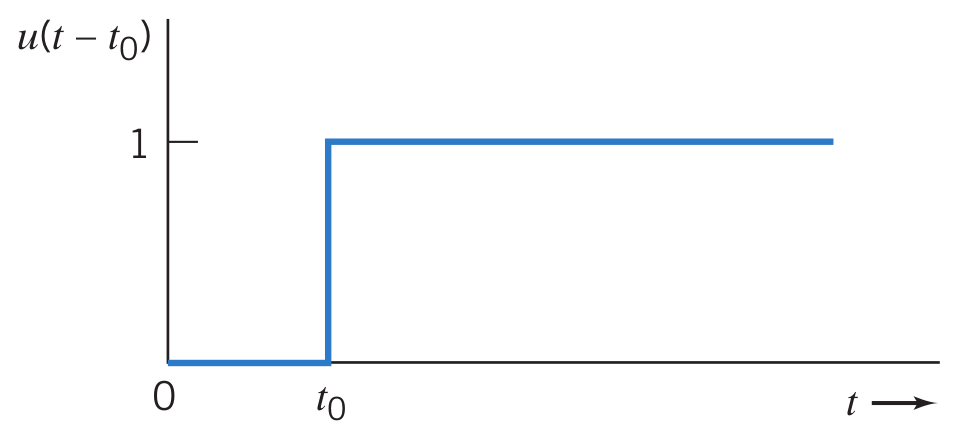
\includegraphics[height=3.2cm]{figure19.png} \newline
\small Unit step forcing function,$ u(t-t_0)$.
		\end{column}
	\end{columns}
\end{tabular}
\end{frame}


% ----------------- NOVO SLIDE --------------------------------
\begin{frame}[fragile]
	\frametitle{The Unit Step Source}
\begin{tabular}{ll}
	\begin{columns}
		\begin{column}{1\textwidth}  %%<--- here
\footnotesize		\textbf{EXERCISE 8.6-2}- Figure below shows a first-order circuit. The input to the circuit is the voltage of
the voltage source, $v_s(t)$. The output is the voltage across the inductor, $v_o(t)$. Determine
the output of this circuit when the input is $v_s(t)=7-14u(t)$ V.
		\begin{center}
    			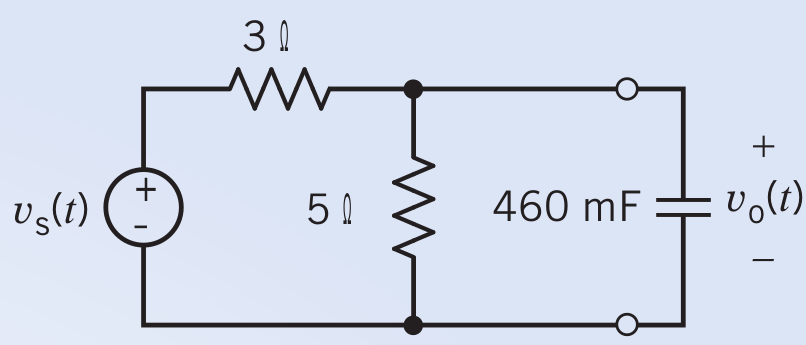
\includegraphics[height=2.5cm]{figure21.png}	
		\end{center}	
	\footnotesize	\scalebox{0.8}{Answer:} $$
	    i_o(t)=
	    \begin{cases}
	    -4.38, \ t<t_0 \\
	    -4.38+8.76e^{-1.16t}V, \ t>t_0\\
	    \end{cases}
	    $$
		\end{column}
	\end{columns}
\end{tabular}
\end{frame}
% ----------------- NOVO SLIDE --------------------------------
\begin{frame}[fragile]
	\frametitle{The Unit Step Source}
\begin{tabular}{ll}
	\begin{columns}
		\begin{column}{1\textwidth}  %%<--- here
\footnotesize		\textbf{EXERCISE 8.6-1}- Figure below shows a first-order circuit. The input to the circuit is the voltage of
the voltage source, $v_s(t)$. The output is the current of the inductor, $i_o(t)$. Determine
the output of this circuit when the input is $v_s(t)=4-8u(t)$ V.
		\begin{center}
    			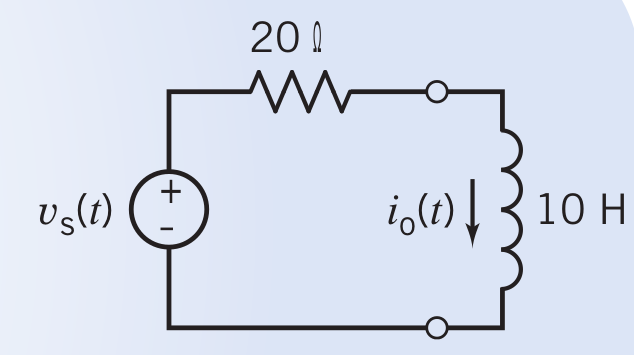
\includegraphics[height=2.5cm]{figure20.png}	
		\end{center}	
	\footnotesize	\scalebox{0.8}{Answer:} $$
	    i_o(t)=
	    \begin{cases}
	    0.2A, \ t<t_0 \\
	    -0.2+0.4e^{-2t}A, \ t>t_0\\
	    \end{cases}
	    $$
		\end{column}
	\end{columns}
\end{tabular}
\end{frame}






% ----------------- NOVA SECÇÂO -----------------------------
\section{The Response of a First-Order Circuit to a Nonconstant Source (8.7)}
% ----------------- NOVO SLIDE --------------------------------
\begin{frame}[fragile]
	\frametitle{Integrating Factor Method}

    		\begin{tabular}{ll}		
    		\begin{columns}
		\begin{column}{1\textwidth}  %%<--- here
 In this section, we introduce the integrating factor method
		\end{column}
	        \end{columns}\\	
	\begin{columns}
	  \begin{column}{.4\textwidth}  %%<--- here
		\begin{eqnarray}
		&&General \ form \ (GF) \nonumber\\
		&&\frac{d}{dt}y(t)+ay(t)=x(t) \nonumber \\
		&&Multiply \ GF \ by\ e^at \nonumber\\ 
		&&( \frac{d}{dt}y+ay )e^{at}=xe^{at} \nonumber \\  
		&&However \nonumber\\
		&&\frac{d(ye^{at})}{dt}=\frac{dy}{dt}e^{at}+aye^{at} \nonumber \\
		 \nonumber	
		 \end{eqnarray}
	  \end{column}
	  \begin{column}{.7\textwidth}  %%<--- here
		\begin{eqnarray}
		&&\frac{d(ye^{at})}{dt}=(\frac{d}{dy}y+ay)e^{at} \nonumber \\ 
		&&Therefore \nonumber\\
		&&\frac{d(ye^{at})}{dt}=xe^{at} \nonumber \\
		&&ye^{at}= \int xe^{at}dt+K \nonumber \\
		&&y(t)=e^{-at} \int xe^{at}dt+Ke^{-at} 	
		 \end{eqnarray}


	  \end{column}
	\end{columns}
\end{tabular}	

\end{frame}
% ----------------- NOVO SLIDE --------------------------------
\begin{frame}[fragile]
	\frametitle{Integrating Factor Method}

    		\begin{tabular}{ll}		
    		\begin{columns}
		\begin{column}{1\textwidth}  %%<--- here
\small The solution of the differential equation $\frac{d}{dt}y(t)+ay(t)=x(t)$ is $y(t)=e^{-at} \int xe^{at}dt+Ke^{-at}$. \newline
		\end{column}
	        \end{columns}\\	
	\begin{columns}
	  \begin{column}{.5\textwidth}  %%<--- here
\small 	  When the source is a constant so that $x(t)=M$, we have
		\begin{eqnarray}
		&&y(t)=e^{-at} \int Me^{at}dt+Ke^{-at} \nonumber\\
		&&y(t)=e^{-at}M \int e^{at}dt+Ke^{-at} \nonumber\\
		&&y(t)=\frac{M}{a}+Ke^{-at} \nonumber\\
		&&y(t)=y_f+y_n \nonumber\\
		 \nonumber	
		 \end{eqnarray}
	  \end{column}
	  \begin{column}{.5\textwidth}  %%<--- here
\small 	  When the source is an exponential so that $x(t)=Me^{bt}$, we have
		\begin{eqnarray}
		&&y(t)=e^{-at} \int Me^{bt}e^{at}dt+Ke^{-at} \nonumber\\
		&&y(t)=Me^{-at}\int e^{(a+b)t}dt+Ke^{-at} \nonumber\\
		&&y(t)=\frac{Me^{bt}}{a+b}+Ke^{-at} \nonumber\\
		&&y(t)=y_f+y_n \nonumber\\
		 \nonumber	
		 \end{eqnarray}
	  \end{column}
	\end{columns}
\end{tabular}	

\end{frame}

% ----------------- NOVO SLIDE --------------------------------
\begin{frame}[fragile]
	\frametitle{The Response of a First-Order Circuit to a Nonconstant Source}
\begin{tabular}{ll}
	\begin{columns}
		\begin{column}{1\textwidth}  %%<--- here
\footnotesize		\textbf{EXERCISE 8.7-1}- Find the current $i$ for the circuit of Figure below for $t>0$ when
$v_s=10e^{-2t}u(t)V$.Assume the circuit is in steady state at $t=0^-$.
		\begin{center}
    			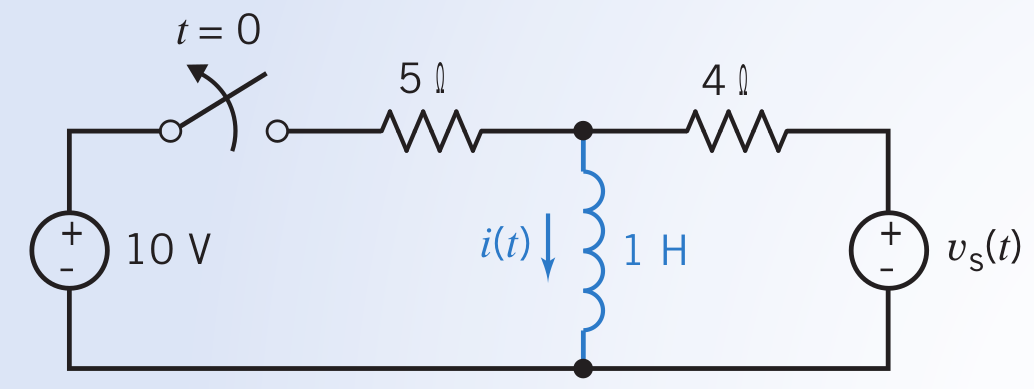
\includegraphics[height=3.5cm]{figure22.png}	
		\end{center}	
	\footnotesize	\scalebox{0.8}{Answer:} $i(t)=-3e^{-4t}+5e^{-2t}A \ t>0$ . 
		\end{column}
	\end{columns}
\end{tabular}
\end{frame}

% ----------------- NOVO SLIDE --------------------------------
\begin{frame}[fragile]
	\frametitle{The Response of a First-Order Circuit to a Nonconstant Source}
\begin{tabular}{ll}
	\begin{columns}
		\begin{column}{1\textwidth}  %%<--- here
\footnotesize		\textbf{EXERCISE 8.7-2}- Find the response $v(t)$ for $t > 0$ for the circuit of Figure below. 
The initial voltage $v(0)=0$, and the current source $i(t)_s=10 \sin (2t)u(t) A$.
		\begin{center}
    			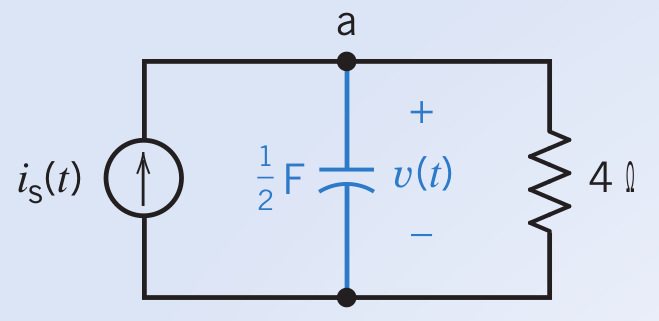
\includegraphics[height=3.5cm]{figure23.png}	
		\end{center}	
	\footnotesize	\scalebox{0.8}{Answer:} $v(t)=\frac{160}{17}e^{-\frac{t}{2}}+\frac{40}{17}\sin(2t)-\frac{160}{17}\cos(2t)V \ t>0$ . 
		\end{column}
	\end{columns}
\end{tabular}
\end{frame}


\end{document} 

